\documentclass[tikz,border=4pt]{standalone}
% Paleta y fuentes compartidas por el libro y las figuras (única fuente de verdad).
\RequirePackage{xcolor}
\definecolor{oxido}{HTML}{B7410E}
\definecolor{cobre}{HTML}{D27D2D}
\definecolor{carbon}{HTML}{2B2B2B}
\definecolor{azul}{HTML}{1F5F8B}
\definecolor{arena}{HTML}{F4EDE4}

\usepackage{fontspec}
\setsansfont{FiraSans}[Extension=.otf,UprightFont=*-Regular,BoldFont=*-SemiBold,ItalicFont=*-Italic,BoldItalicFont=*-SemiBoldItalic]
\setmonofont{FiraMono}[Extension=.otf,UprightFont=*-Regular,BoldFont=*-Medium,Scale=0.95]
\usetikzlibrary{positioning,arrows.meta,calc}
\begin{document}
\sffamily\small
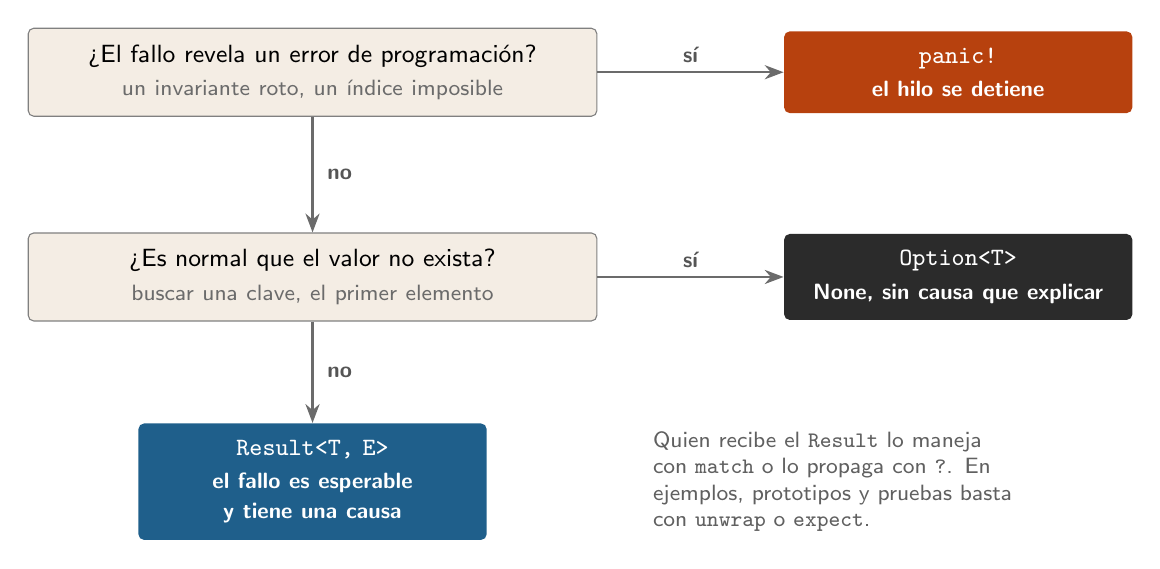
\begin{tikzpicture}[>={Stealth[length=2.4mm]},
  execute at begin node={\hyphenpenalty=10000},
  preg/.style={draw=carbon!60,fill=arena,rounded corners=2pt,align=center,
    text width=68mm,inner sep=6pt,font=\sffamily\small},
  resp/.style={rounded corners=2pt,align=center,text width=40mm,inner sep=6pt,
    font=\sffamily\small,text=white},
  eti/.style={font=\sffamily\footnotesize\bfseries,text=carbon!80,inner sep=2pt},
  nota/.style={font=\sffamily\footnotesize,text=carbon!75,align=left}]
  \node[preg] (q1) at (0,0) {¿El fallo revela un error de programación?\\[1pt]
    {\footnotesize\color{carbon!70}un invariante roto, un índice imposible}};
  \node[preg] (q2) at (0,-2.6) {¿Es normal que el valor no exista?\\[1pt]
    {\footnotesize\color{carbon!70}buscar una clave, el primer elemento}};
  \node[resp,fill=azul] (r) at (0,-5.2) {\ttfamily\bfseries Result<T, E>\\[1pt]
    \sffamily\footnotesize el fallo es esperable y tiene una causa};
  \node[resp,fill=oxido] (p) at (8.2,0) {\ttfamily\bfseries panic!\\[1pt]
    \sffamily\footnotesize el hilo se detiene};
  \node[resp,fill=carbon] (o) at (8.2,-2.6) {\ttfamily\bfseries Option<T>\\[1pt]
    \sffamily\footnotesize None, sin causa que explicar};
  \draw[->,thick,carbon!70] (q1) -- node[eti,above=1pt] {sí} (p);
  \draw[->,thick,carbon!70] (q2) -- node[eti,above=1pt] {sí} (o);
  \draw[->,thick,carbon!70] (q1) -- node[eti,right=3pt] {no} (q2);
  \draw[->,thick,carbon!70] (q2) -- node[eti,right=3pt] {no} (r);
  \node[nota,anchor=west,text width=50mm] at (4.2,-5.2)
    {Quien recibe el \texttt{Result} lo maneja con \texttt{match} o lo
     propaga con \texttt{?}. En ejemplos, prototipos y pruebas basta
     con \texttt{unwrap} o \texttt{expect}.};
\end{tikzpicture}
\end{document}
